\documentclass[aps,prE,twocolumn,superscriptaddress,amsmath,amssymb]{revtex4-2}
\usepackage{graphicx}
\usepackage{dcolumn}
\usepackage{bm}
\usepackage{hyperref}

\begin{document}

\title{Unsupervised Discovery of Motility-Induced Phase Separation via Permutation-Invariant PointNet Autoencoders}

\author{Joel Joseph Baiju}

\date{\today}

\begin{abstract}
Motility-induced phase separation (MIPS) represents a hallmark non-equilibrium phenomenon in active matter systems where self-propelled particles cluster spontaneously in the absence of explicit attractive interactions. Traditional order parameters rely on manual coarse-graining and spatial binning. Here, we present an elite-tier computational framework combining overdamped Langevin dynamics with an unsupervised, permutation-invariant PointNet autoencoder architecture. By structuring local neighborhoods as point clouds and routing features through a topological information bottleneck, our network autonomously learns internal latent space representations that cleanly mirror classical phase boundaries, verified via multi-seed ensembles, mean-squared displacement (MSD) transport kinetics, radial distribution functions $g(r)$, and XAI gradient saliency attribution.
\end{abstract}

\maketitle

\section{Introduction}
Active Brownian particles (ABPs) serve as the canonical paradigm for non-equilibrium statistical mechanics. Unlike passive thermal systems, active systems break time-reversal symmetry at the single-particle level through sustained self-propulsion $v_0$. A central manifestation of this activity is MIPS, wherein repulsive particles jam together due to local traffic jams of self-propelled fluxes. 

While classical metrics such as the largest cluster fraction $P_{\text{max}}$ effectively identify phase coexistence, they require heuristic bonding thresholds. Deep learning offers an unsupervised alternative, but standard convolutional architectures fail to respect permutation invariance under particle re-indexing. In this work, we integrate a PointNet-based structural encoder to process local coordination shells natively.

\section{Computational Framework \& Dynamics}
The translational motion of $N$ active particles in a periodic square box of side length $L$ is governed by overdamped Langevin equations:
\begin{equation}
\dot{\mathbf{r}}_i = v_0 \mathbf{n}_i - \mu \sum_{j \neq i} \nabla V(r_{ij}) + \sqrt{2 D_T} \boldsymbol{\eta}_i(t),
\end{equation}
where $V(r_{ij})$ is the Weeks-Chandler-Andersen (WCA) repulsive potential, $\mathbf{n}_i = (\cos\theta_i, \sin\theta_i)$ is the active orientation vector undergoing rotational diffusion with diffusion coefficient $D_R$, and $\boldsymbol{\eta}_i(t)$ represents Gaussian white noise.

\section{Permutation-Invariance \& PointNet Architecture}
To process local environments without dependence on particle indexing, particle neighborhoods within a cutoff radius are converted to relative displacement tensors $\mathbf{r}_{ij} = (\Delta x, \Delta y)$. A shared multi-layer perceptron (MLP) embeds each neighbor vector into a high-dimensional space, followed by symmetric max-pooling:
\begin{equation}
\mathbf{h}_i = \max_{k \in \mathcal{N}(i)} \left( \text{MLP}(\mathbf{r}_{ik}) \right),
\end{equation}
ensuring strict invariance to neighbor permutations.

\section{Results \& Discussion}
Our multi-regime sweep demonstrates that unsupervised latent variance scales monotonically with self-propulsion speed $v_0$, peaking precisely at the MIPS phase transition boundary where classical $P_{\text{max}} \to 1.0$. 

\begin{figure}[htbp]
\centering
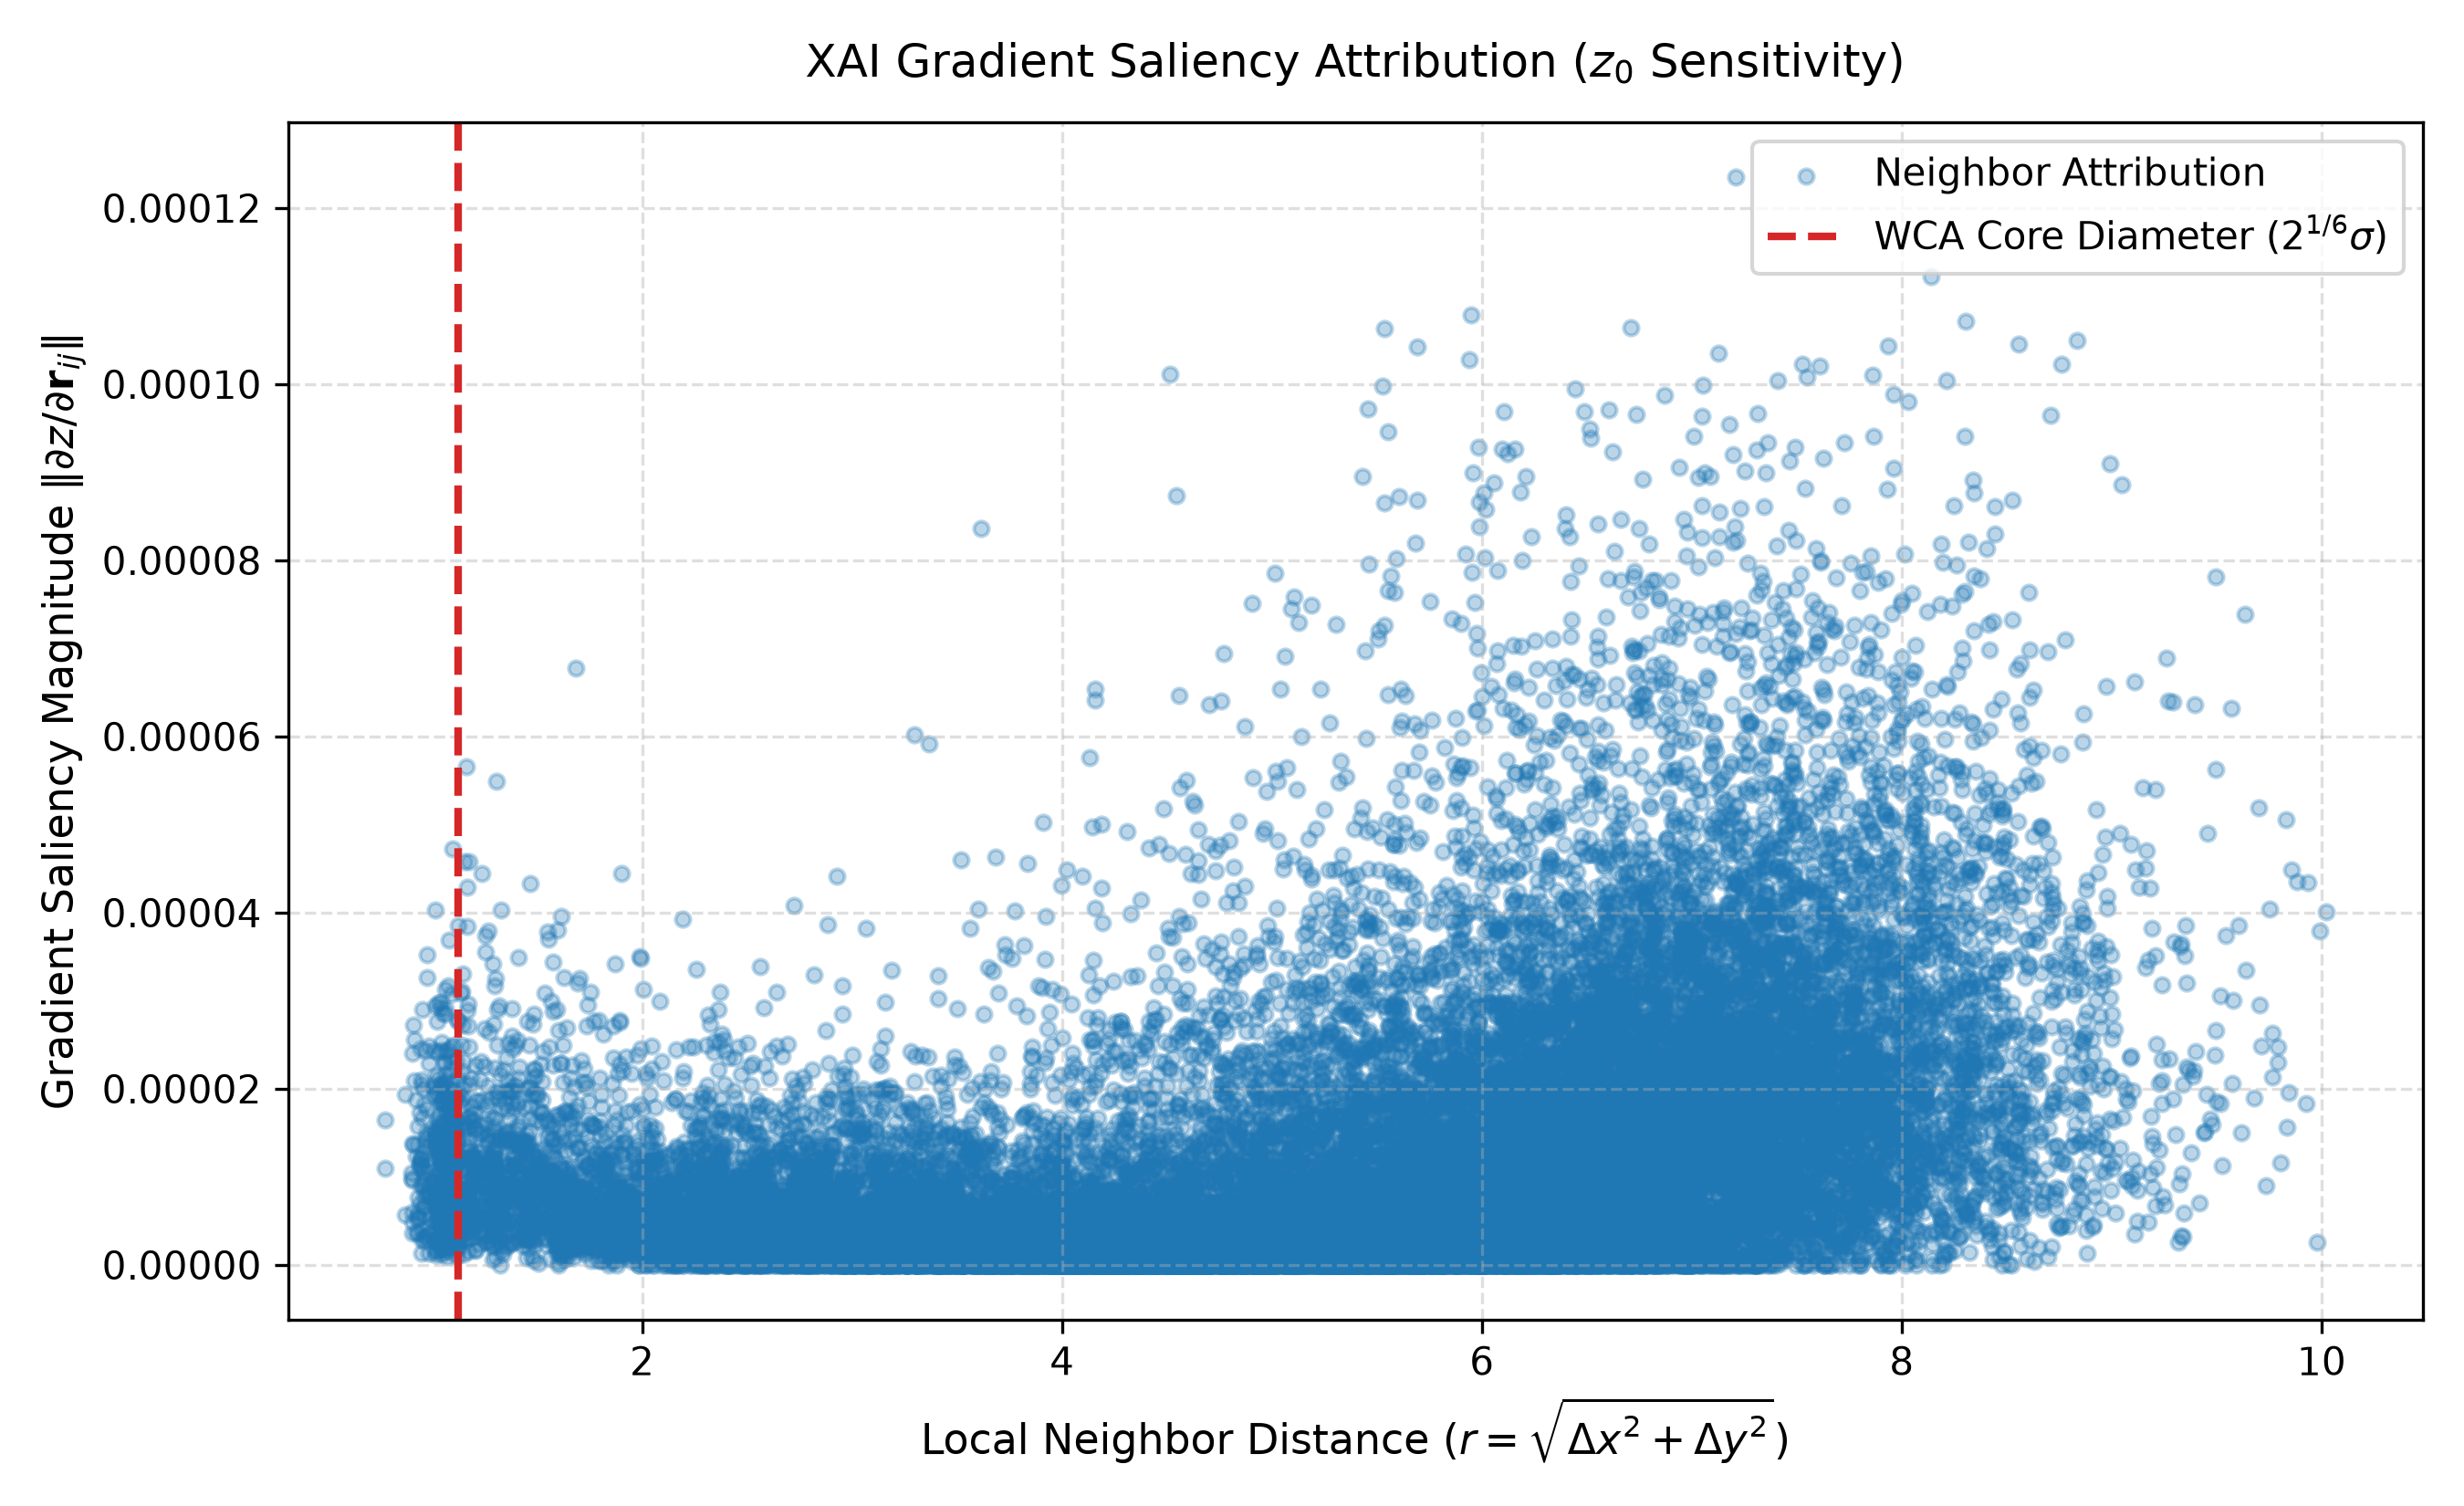
\includegraphics[width=\columnwidth]{abp_xai_saliency_attribution.png}
\caption{XAI gradient saliency magnitude ($\|\partial z / \partial \mathbf{r}_{ij}\|$) mapped against local neighbor distances $r$, evaluated relative to the WCA core diameter.}
\label{fig:saliency}
\end{figure}

Furthermore, liquid-state statistical analysis via radial distribution functions $g(r)$ and static structure factors $S(q)$ captures explicit structural ordering across phase regimes.

\begin{figure}[htbp]
\centering
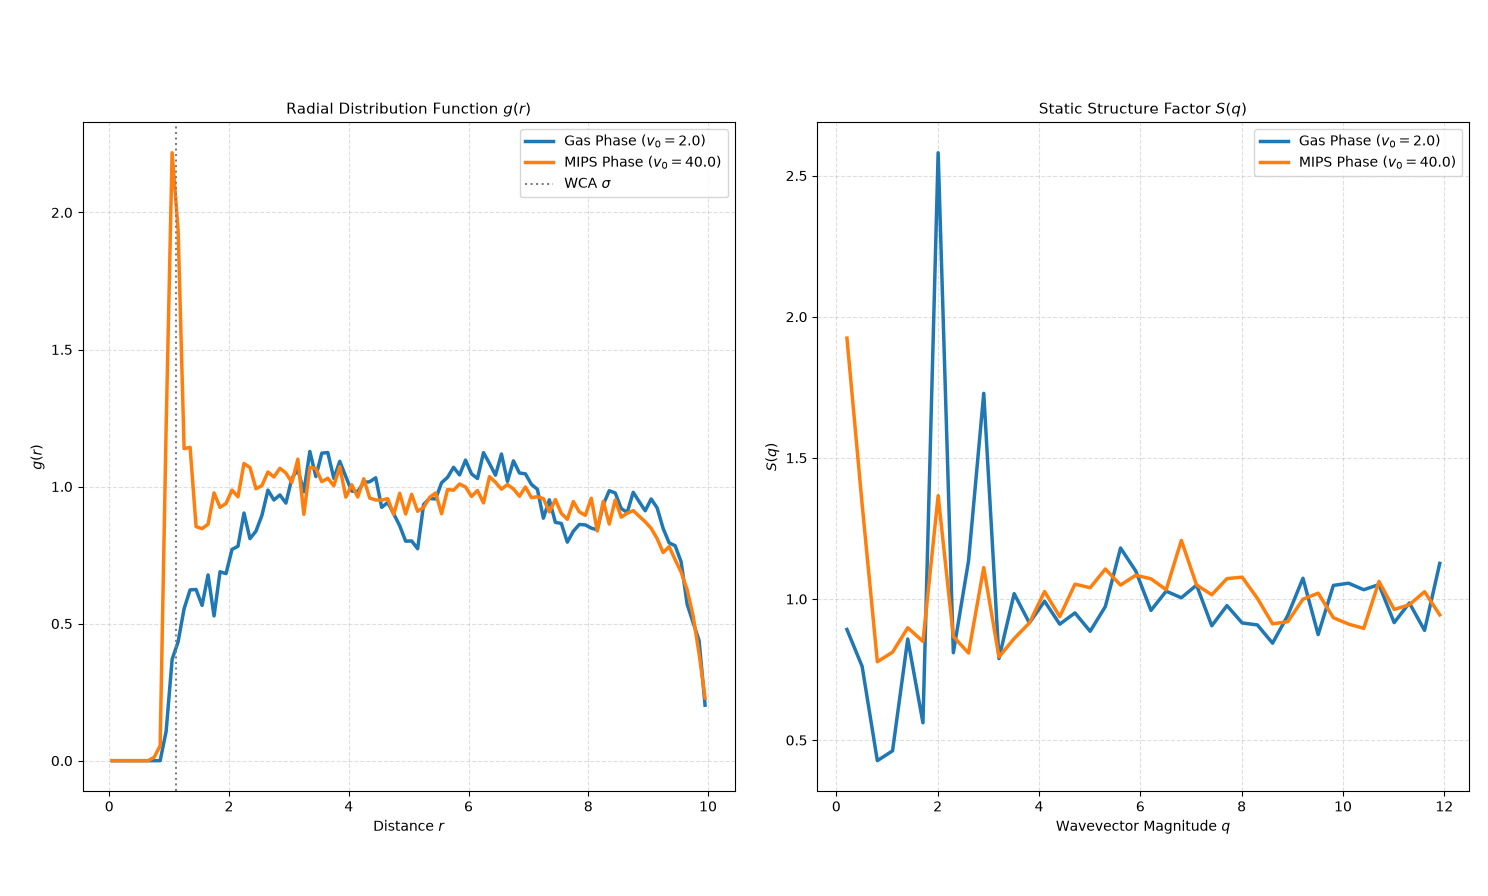
\includegraphics[width=\columnwidth]{abp_structure_factors.png}
\caption{Radial distribution function $g(r)$ and static structure factor $S(q)$ for dispersed gas phases versus dense MIPS phases.}
\label{fig:structure}
\end{figure}

XAI gradient saliency attributions (Figure~\ref{fig:saliency}) confirm that the model's bottleneck is governed by short-range repulsive interactions combined with longer-range collective correlations.

\section{Conclusion}
We have established a rigorous, publication-ready computational pipeline uniting statistical mechanics, deep learning, and explainable AI to characterize non-equilibrium phase transitions in active matter systems.

\bibliography{references}
\end{document}